\chapter{Volumetric Properties of Pure Substances}\label{Chapter:VolumetricPropertiesPureSubstances}

   \begin{LearningObjectivesBlock}{Learning Objectives}
      Upon completion of this chapter, you will be able to
        \begin{enumerate}
           \item Define pure substances and thermodynamic phases;
           \item State the Gibbs phase rule and its use to define the number of degrees of freedom of a system;
           \item Identify phases and phase transitions in a diagram;
           \item Formulate the solution for thermodynamic problems involving the calculation of volume of pure substances;
           \item Select appropriate equation of state for a given problem/application;
        \end{enumerate}
\medskip
     Recommended reading: Chapters 3 of \citet{SmithVanNess_Book}, 6 of \citet{Sandler_Book}, 2 of \citet{Borgnakke_Book}, 11 of \citet{Moran_Book} or 4 of \citet{Atkins_Book}.
   \end{LearningObjectivesBlock}


%%%%%%%%%%%%%%%%%%%%%%%%%%%%%%%%%%%%%%%%%%%%%%%%%%%%%%%%%%%%%%%%%
\begin{comment}
   \begin{LearningObjectivesBlock}{Learning Objectives}
      Upon completion of this chapter, you will be able to
        \begin{enumerate}
           \item {\bf Knowledge:} Define, Name, Select, State 
           \item {\bf Comprehension:} Describe, Identify, Discuss
           \item {\bf Application:} Apply, Demonstrate, Employ, Sketch
           \item {\bf Analysis:} Analyse, Compare, Calculate, Solve
           \item {\bf Synthesis:} Determine, Formulate
           \item {\bf Evaluation:} Assess, Check, Estimate, Compare, Measure, Monitor
        \end{enumerate}
\end{comment}
%%%%%%%%%%%%%%%%%%%%%%%%%%%%%%%%%%%%%%%%%%%%%%%%%%%%%%%%%%%%%%%%%
  

%%%% ETOC
\localtableofcontents

%%%
%%% SECTION
%%%
   \section{Introduction}\label{Chapter:VolumetricPropertiesPureSubstances:Section:Intro}
   Definitions and assumptions for ideal gas behaviour were introduced in Section~\ref{Chapter:Intro_Property_of_Gases:Section:IdealGases} along with the corresponding equation of state (Eqn.~\ref{Chapter:Intro_Property_of_Gases:Eqn:IdealEOS}). A fluid behaves as an ideal gas at low to moderate pressure (often below atmospheric pressure) and at high temperatures. Under different conditions, fluids may not behave as ideal gases and therefore other equations of state (not just for gases) were designed to describe the {\it PVT} behaviour of fluids.

Phase transition of pure substances is one of the main topics in industrial chemical engineering as it is of paramount importance to calculate fluid properties for the design of equipment and processes. Therefore, the main aim of this chapter is to introduce the concept of phase diagram of pure substances and its mathematical representation as equations of state. 

  
%%%
%%% SECTION
%%%
   \section{Phase Diagrams of Pure Substances}\label{Chapter:VolumetricPropertiesPureSubstances:Section:PhaseDiagrams}\index{Phase diagram}\index{Triple point}\index{Supercritical state}

Pure substances/fluids can be defined as materials of homogeneous and constant composition. For example, systems containing water-ice, water-steam or water-ice-steam are considered pure fluids (or substances) at different phases, whereas (a) air-water, (b) air-steam and (c) gaseous mixture containing N$_{2}$, H$_{2}$, O$_{2}$ and NO$_{2}$ are considered as either homogeneous (b-c) or heterogeneous (a) mixtures.

A pure substance can exist and coexist in different phases\footnote{Phase of a substance can be defined as the form of matter that is uniform in chemical composition and physical state.}  (\ie solid, liquid and vapour -- S, L and V). Phase behaviour of substances is often represented by {\it PVT}\footnote{{\it PVT} stands for pressure, specific (or molar) volume and temperature.} phase diagrams that describe phase transitions (\ie spontaneous conversion -- or mass/heat transfer of one phase to another) and coordinates. A 3D {\it PVT} diagram of an arbitrary substance is shown in Figure~\ref{Chapter:VolumetricPropertiesPureSubstances:Fig:PVT_Surfaces}a, where solid, liquid and vapour phases are represented by continuous volumes and, the regions between these volumes are representations of phase equilibrium, \ie regions where phases coexist in thermodynamic equilibrium.

   %%% FIGURE
           \begin{figure}[h]
              \begin{center}
                 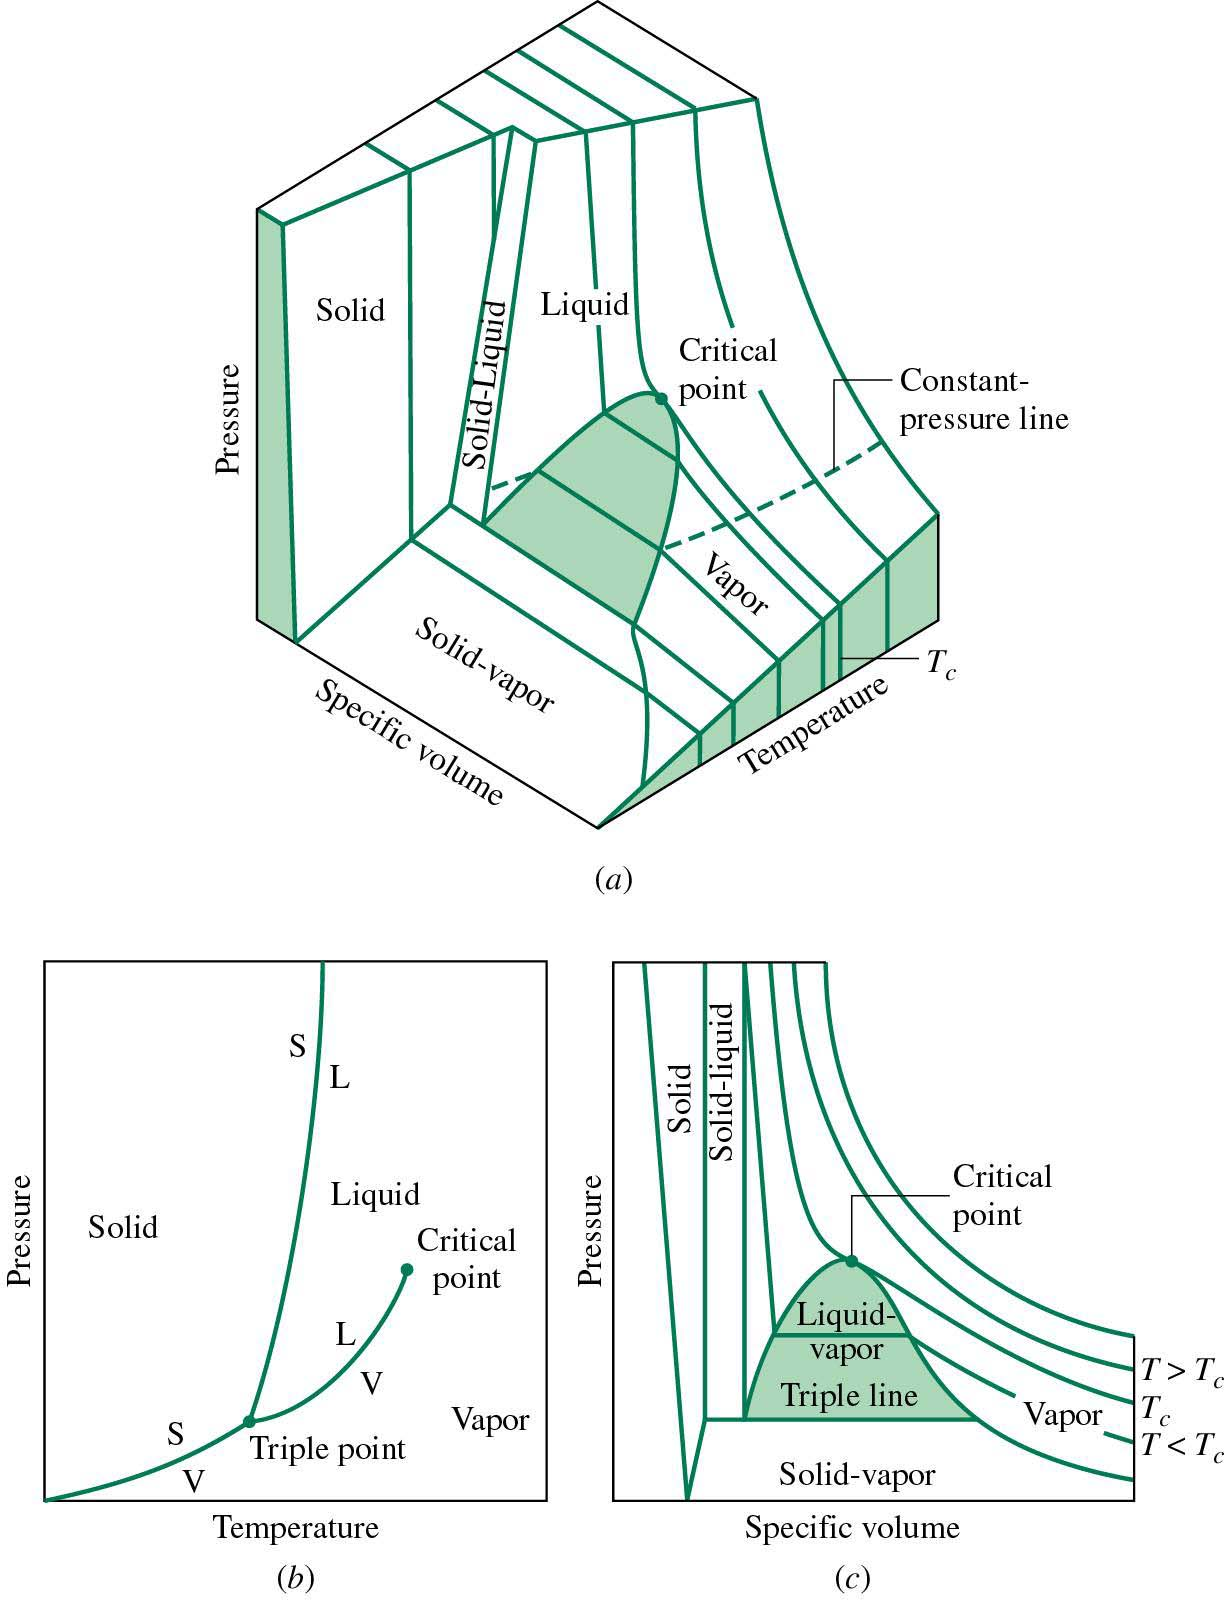
\includegraphics[width=10.cm,clip]{./Figs/PVT_Surface.jpg}
                 \caption{$PVT$ volume (top) and projections onto (b) $PT$ and (c) $PV$ diagrams for a pure substance \citep[Extracted from][]{Borgnakke_Book}.}\label{Chapter:VolumetricPropertiesPureSubstances:Fig:PVT_Surfaces}
              \end{center}
           \end{figure}    

Such 3D representation helps determining (qualitatively) phases (S, L and V) at prescribed coordinates (temperature, specific/molar volume and pressure) of fluids. However, it is not convenient dealing with 3D plots and, most of the time, we may want to extract quantitative values of fluids (Chapter~\ref{Chapter:ThermodynamicPropertiesPureFluids}). A better approach is to project 3D plots into surfaces, \ie through $PT$, $PV$ and $VT$ phase diagrams as shown in Figs.~\ref{Chapter:VolumetricPropertiesPureSubstances:Fig:PVT_Surfaces}b and \ref{Chapter:VolumetricPropertiesPureSubstances:Fig:PVT_Surfaces}c.

$PV$ diagram (Fig.~\ref{Chapter:VolumetricPropertiesPureSubstances:Fig:PV-PT_Diagrams}a) is a representation of the PVT volume, Fig.~\ref{Chapter:VolumetricPropertiesPureSubstances:Fig:PVT_Surfaces}a, where surfaces (\ie areas) represent both single phases and phases in equilibrium, and lines represent transition between phases. Here, there are three properties that we need to define:
           \begin{enumerate}[a)]
              \item Critical point (or state): coordinates in which two phases of a fluid become indistinguishable. Beyond this coordinate, a fluid is neither completely liquid nor completely gaseous, \ie exhibits properties of both the liquid phase and the gas phase and is referred to as a {\it supercritical fluid}. All fluids have distinct critical coordinates, known as {\it critical pressure} $\left(\text{P}_{c}\right)$, {\it critical temperature} $\left(\text{T}_{c}\right)$ and {\it critical volume} $\left(\text{V}_{c}\right)$. Interesting videos about critical state can be seen in 
                  \begin{center}
                     \href{https://www.youtube.com/watch?v=bJjcTpRzXpM}{https://www.youtube.com/watch?v=bJjcTpRzXpM} and \\
                     \href{https://www.youtube.com/watch?v=RmaJVxafesU}{https://www.youtube.com/watch?v=RmaJVxafesU}.
                  \end{center}
              \item Saturation lines (blue lines in Fig.~\ref{Chapter:VolumetricPropertiesPureSubstances:Fig:PV-PT_Diagrams}a) are coordinates in which phase transition starts to occur.
              \item Isotherms: Lines of constant temperature.
           \end{enumerate}

   %%% FIGURE
           \begin{figure}[h]
              \vbox{
                    \hbox{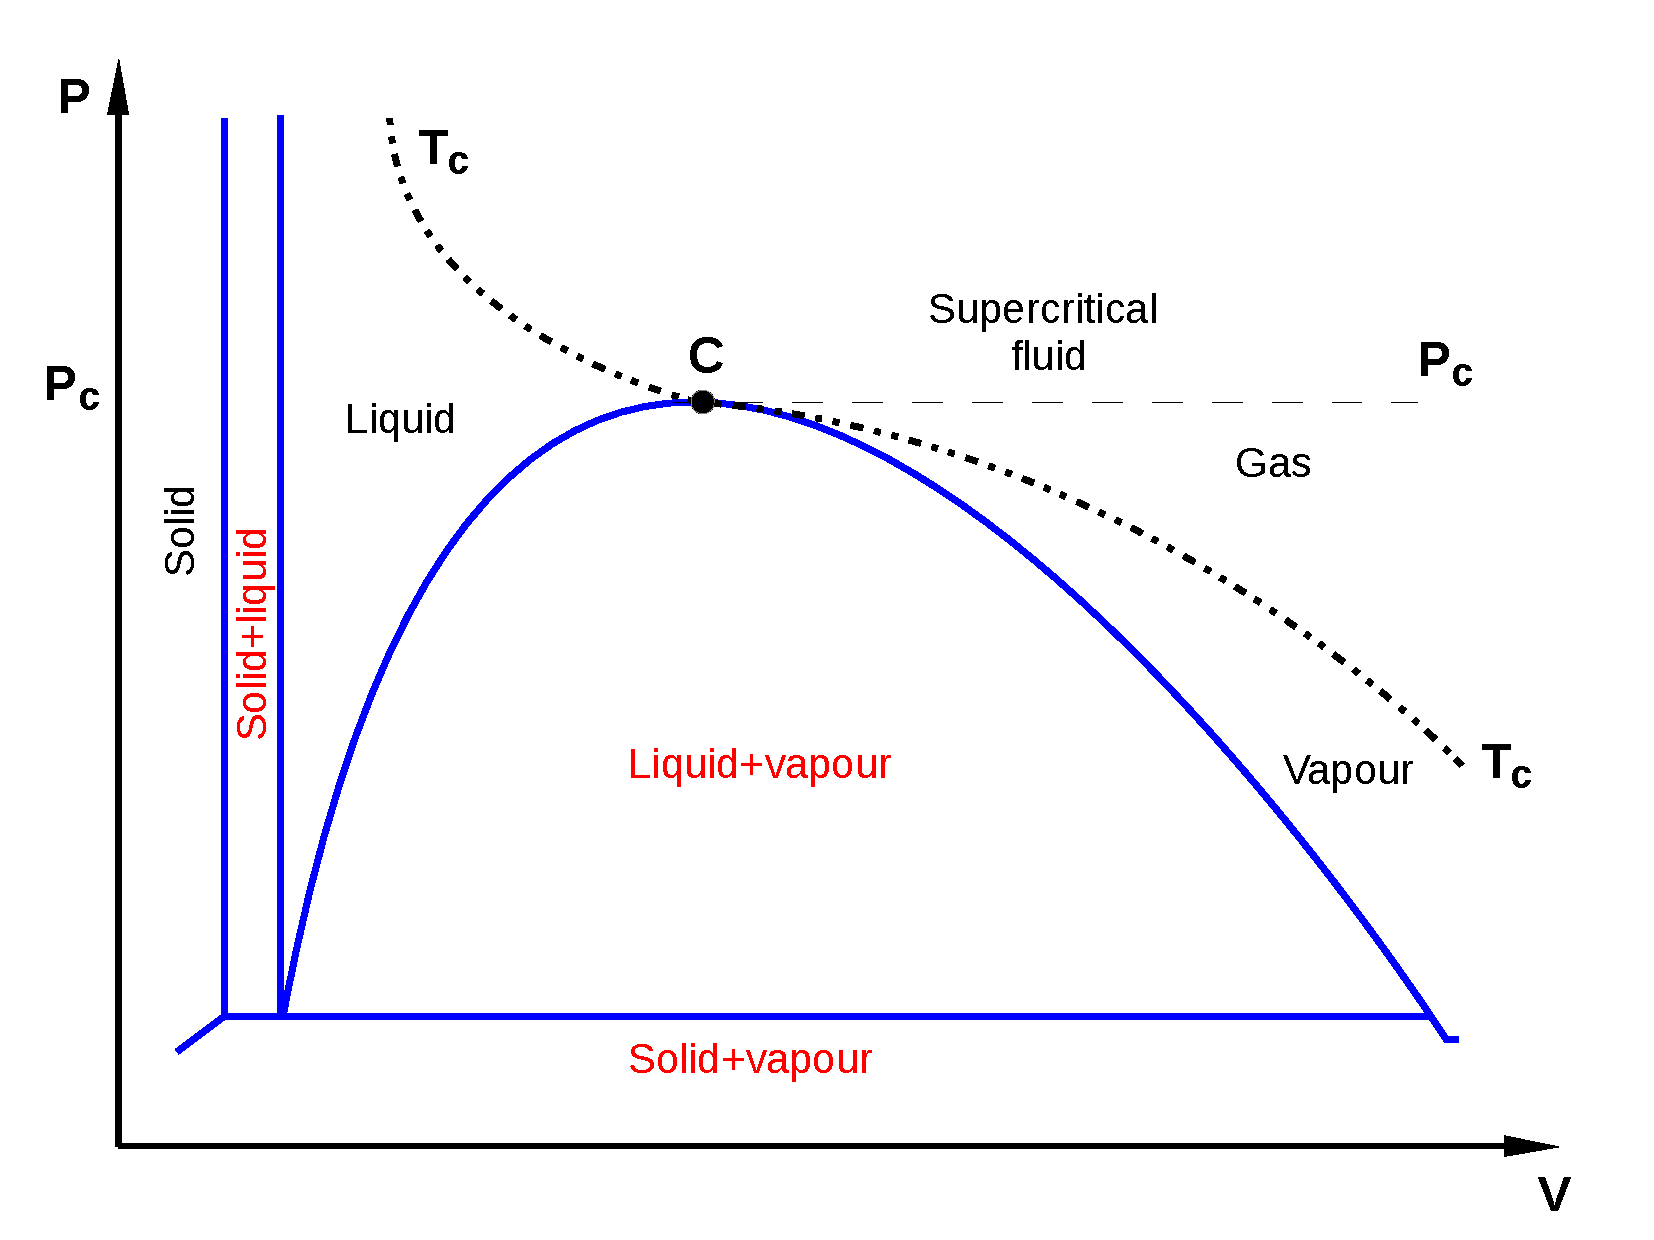
\includegraphics[width=.5\columnwidth,clip]{./Figs/PV_Diagram1}
                          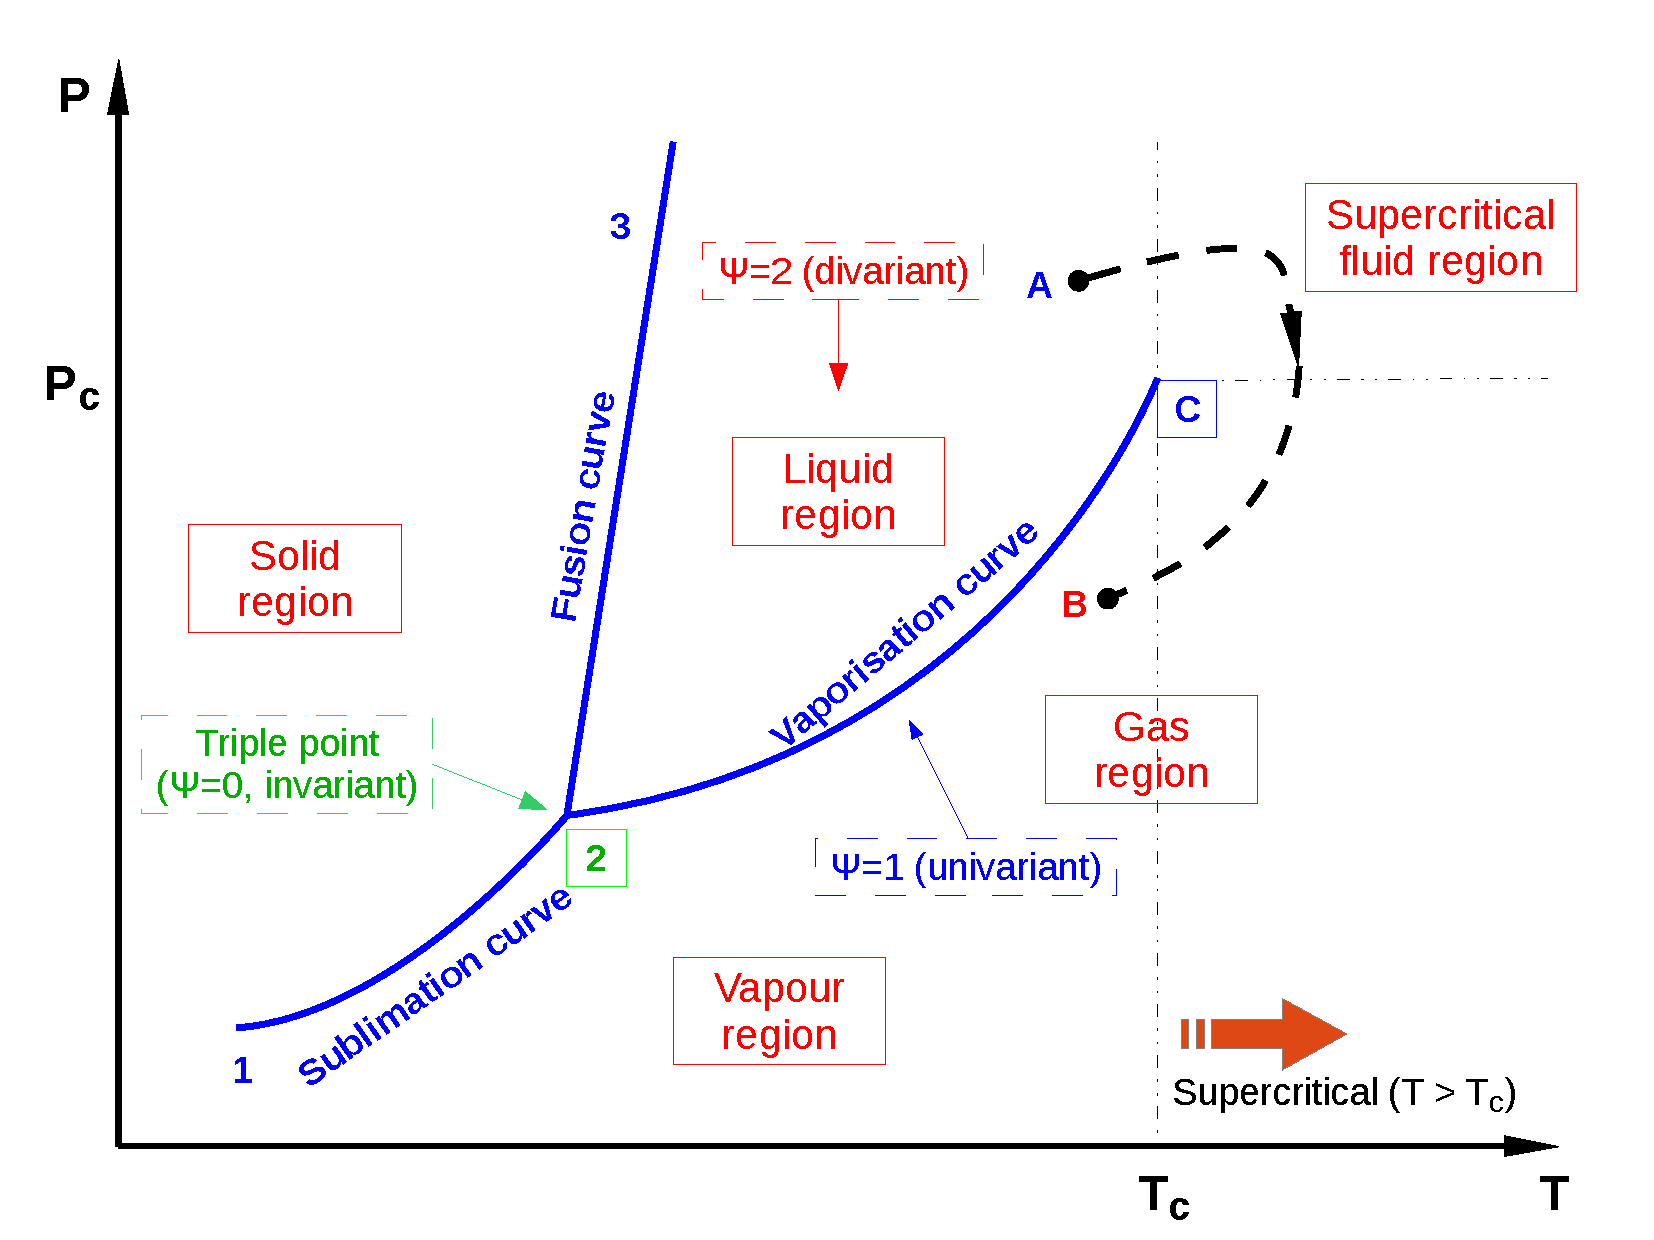
\includegraphics[width=.5\columnwidth,clip]{./Figs/PT_Diagram}}
                    \vspace{-.1cm}
                    \hbox{\hspace{4cm}(a)\hspace{8cm}(b)}}
              \caption{ (a) $PV$ and (b) $PT$ diagrams for a pure substance. Dotted line in (a) represents the isotherm at T=T$_{c}$.}\label{Chapter:VolumetricPropertiesPureSubstances:Fig:PV-PT_Diagrams}
           \end{figure}


           In vapour-liquid equilibrium (VLE) systems there are two main saturation lines: {\it saturated liquid line} (left-hand side of $C$ in Fig.~\ref{Chapter:VolumetricPropertiesPureSubstances:Fig:PV-PT_Diagrams}a)  and {\it saturated vapour line} (rhs of $C$) that represent the initial transition from a single phase system to a two or three phases system. 
%

$PT$ diagrams (Fig.~\ref{Chapter:VolumetricPropertiesPureSubstances:Fig:PV-PT_Diagrams}b) are representations of Fig.~\ref{Chapter:VolumetricPropertiesPureSubstances:Fig:PVT_Surfaces}a, where phases are defined by surfaces (\ie areas) with continuous lines representing phases transitions (\ie in equilibrium). The {\it triple point} is coordinate in which all three phases (S, L and V) coexist in equilibrium.

A fluid in the compressed liquid state is often called {\it sub-cooled fluid} (central region of Fig.~\ref{Chapter:VolumetricPropertiesPureSubstances:Fig:PV-PT_Diagrams}b), while a gas at a pressure lower than its saturation vapour pressure for a given temperature is said to be at {\it superheated state}.


%%% SECTION
%%%
\section{Gibbs Phase Rule}\label{Chapter:VolumetricPropertiesPureSubstances:Section:GibbsPhaseRule}\index{Phase rule}\index{Gibbs phase rule|see {Phase rule}}\index{Phase rule !Degrees of freedom}\index{Degrees of freedom|see {Phase rule}}
  In the $PT$ diagram (Fig.~\ref{Chapter:VolumetricPropertiesPureSubstances:Fig:PV-PT_Diagrams}b) of an arbirtrary pure substance, three regions may be clearly noted, liquid, vapor and solid. In order to fix any of such thermodynamic states, both temperature and pressure are needed, \ie a one-component, single phase system has two {\it degrees of freedom}. However, during phase transition (\eg vaporisation , fusion or sublimation lines), any change in pressure will lead to change in temperature in order to fix the thermodynamic state. Therefore, it is important to obtain precise information to set up a thermodynamic state of a multi-component and multiphase system.

  Let's consider a non-reactive system in equilibrium within $\mathcal{P}$ phases  (\ie $L$, $V$ and/or $S$) containing $\mathcal{C}$ independent chemical species.  The number of degrees of freedom $\left(\Psi\right)$ for the system (\ie the number of intensive variables that may vary independently) may be expressed as,
  \begin{shaded}
    \begin{center}
      Degrees of freedom = (Number of state variables) – (Number of independent equations),
    \end{center}
    \noindent where
    \begin{itemize}
       \item Number of intensive variables: $T$, $P$ and $\left(\mathcal{C}-1\right)$ species mole fractions for each of the $\mathcal{P}$ phases;
        \item Number of independent equations: $\left(\mathcal{C}-1\right)\mathcal{N}$;
    \end{itemize}
    therefore, the phase rule may be rewritten as
    \begin{eqnarray}
       \Psi &=& \left[2 + \left(\mathcal{C}-1\right)\mathcal{P}\right] - \left[\left(\mathcal{P}-1\right)\mathcal{C}\right] \nonumber \\
            &=& 2 + \mathcal{C} - \mathcal{P}\label{Chapter:VolumetricPropertiesPureSubstances:Eqn:PhaseRule}
    \end{eqnarray}  
  \end{shaded}
  The Gibbs phase rule is a relation that determines the number of independent variables that must be specified to establish the intensive state of any system at equilibrium. The degrees of freedom (\ie number of intensive properties such as temperature and pressure) determines the number of variables that must be specified to fix all other remaining phase rule variables. 

For example, for a pure liquid component, the phase rule yields two degrees of freedom, \ie if temperature and pressure are specified, all other intensive properties (\eg enthalpy, entropy etc) are uniquely determined. However, if the same liquid component is in equilibrium with its vapour phase (\eg water and steam) there is {\it only} one degree of freedom. This means that either pressure or temperature may be specified to fix all other intensive properties of the system. At the triple point the number of degrees of freedom is {\it zero}, \ie any change from such state (\eg for water-steam-ice at 273.16 K and 0.006112 bar) causes at least one of the phases to vanish.


%%% SECTION
\section{PVT Behaviour of Pure Substances}\label{Chapter:VolumetricPropertiesPureSubstances:Section:PVTBehaviour}\index{Gases!Ideal gas}\index{Equation of State!Ideal gas}
In Section~\ref{Chapter:Intro_Property_of_Gases:Section:IdealGases}, the ideal gas equation of state (EOS) was defined as 
     \begin{displaymath}
        PV = RT,
     \end{displaymath}
     where $V\left(=\frc{V^{t}}{n}\right)$ is the molar volume $\left(\text{V}^{t}\text{ is the total volume and } n \text{ is the number of moles}\right)$ . This is a relationship between macroscopic intensive properties, and is based in two main assumptions \wrt the microscopic behaviour of molecules:
     \begin{enumerate}[(a)]
        \item Molecules have no extension in space (\ie zero volume), and;
        \item Molecules do not interact with each other.
     \end{enumerate}
     The second assumption is particularly important as it considers that atoms and molecules either do not interact or do not have electric charge or have an infinite distance between them (\ie low density conditions). However, these assumptions are rarely met in real conditions (both in the environment and in industry) and several mathematical relations have been developed to better represent the PVT behaviour of real fluids.

\section{Generic Form of Equations of State}\label{Chapter:VolumetricPropertiesPureSubstances:CompressibilityExpansivityCoefficients}\index{Coefficient of thermal expansion}\index{Coefficient of isothermal compressibility}\index{Volume expansivity coefficient|see {Coefficient of thermal expansion}}
 \begin{subequations}
     The PVT behaviour of real pure fluids can be expressed as functional, \ie a generic form of an equation of state,
        \begin{displaymath}
           f(P,V,T) = 0,
        \end{displaymath}
        however, from the Gibbs phase rule for a single phase pure component the number of degrees of freedom is equal to 2. Therefore, we can write this function in its simplest way (or EOS), 
        \begin{displaymath}
           V=V(T,P),
        \end{displaymath}
        or in differential form,
        \begin{displaymath}
            dV = \Partial[V]{T}{P}dT +  \Partial[V]{P}{T}dP
        \end{displaymath}
        \begin{shaded}
           Defining the {\it coefficient of thermal expansion} (or {\it volume expansivity coefficient}), $\beta$, and the {\it coefficient of isothermal compressibility}, $\kappa$ as,
           \begin{equation}
               \beta \equiv \frc{1}{V}\Partial[V]{T}{P}\;\;\;\text{ and }\;\;\; \kappa \equiv -\frc{1}{V}\Partial[V]{P}{T}\label{Chapter:VolumetricPropertiesPureSubstances:Eqn:CompressibilityExpansivity}
           \end{equation}
           respectively, leading to
           \begin{equation}
              \frc{dV}{V} = \beta dT - \kappa dP.\label{Chapter:VolumetricPropertiesPureSubstances:Eqn:CompressibilityExpansivity2}
           \end{equation}
        \end{shaded}
 \end{subequations}

   % Example
   \begin{MyExample}{\begin{center}{\bf Example}\end{center}}
     \begin{example}\label{Chapter:VolumetricPropertiesPureSubstances:Example1}
         Derive the relations for coefficient of thermal expansion and the isothermal compressibility coefficient for
              \begin{enumerate}[(a)]
                  \item Ideal gas EOS;
                  \item $V=\frc{a}{RT}+\frc{bT}{PR}$ 
              \end{enumerate}
     \end{example}

% SOLUTION
       \noindent{\bf Solution:}
         Here we need to obtain expressions for 
           \begin{eqnarray}
                && \beta = \frc{1}{V}\left(\frc{\partial V}{\partial T}\right)_{P} \nonumber \\
                && \kappa = -\frc{1}{V}\left(\frc{\partial V}{\partial P}\right)_{T} \nonumber
           \end{eqnarray}
           for 
           \begin{enumerate}[a)]
%
               \item Ideal gas EOS, $V=\frc{R T}{P}$,
                    \begin{displaymath}
                       \beta =\frc{P}{R T}\frc{R}{P} = \frc{1}{T},
                    \end{displaymath}
                    and 
                    \begin{displaymath}
                       \kappa = -\frc{P}{R T}\left(-\frc{R T}{P^{2}}\right) = \frc{1}{P}
                    \end{displaymath}
%
               \item $V=\frc{a}{RT}+\frc{bT}{PR}$: Solving the partial differentials,
                    \begin{displaymath}
                       \left(\frc{\partial V}{\partial T}\right)_{P} = \frc{b}{PR}-\frc{a}{RT^{2}}\;\;\text{ and }\;\; \left(\frc{\partial V}{\partial P}\right)_{T} = -\frc{bT}{P^{2}R},
                    \end{displaymath}
                    thus
                    \begin{eqnarray}
                       && \beta =\frc{1}{\frc{a}{RT}+\frc{bT}{PR}}\left(\frc{b}{PR}-\frc{a}{RT^{2}}\right) = \frc{\frc{bT^{2}-aP}{PRT^{2}}}{\frc{aP+bT^{2}}{PRT}} = \frc{bT^{2}-aP}{T\left(aP+bT^{2}\right)}
 \nonumber \\
                       && \kappa = -\frc{1}{\frc{a}{RT}+\frc{bT}{PR}} \left(-\frc{bT}{P^{2}R}\right) = \frc{bT^{2}}{P\left(aP+bT^{2}\right)} \nonumber
                    \end{eqnarray}           
           \end{enumerate}
   \end{MyExample}
   

\section{The Virial Equation of State}\label{Chapter:VolumetricPropertiesPureSubstances:VirialEOS}\index{Equation of State!Virial}\index{Compressibility factor|see {Equation of State}} \index{$Z$|see {Compressibility factor}}\index{Equation of State!Compressibility factor}
 \begin{subequations}
     The Virial EOS was introduced by H. Kamerlingh-Omnes in 1901 to describe gas compressibily coefficient, $Z$, as a power series  in terms of $\frac{1}{V}$ for a pure gas, with two alternate forms:
       \begin{eqnarray}
          \frc{P V}{R T} &=& 1 + \frc{B}{V} + \frc{C}{V^{2}} + \cdots \text{ or} \label{Chapter:VolumetricPropertiesPureSubstances:Eqn:Virial1}\\
          \frc{P V}{R T} &=& 1 + B^{\prime}P + C^{\prime}P^{2} + \cdots,\label{Chapter:VolumetricPropertiesPureSubstances:Eqn:Virial2} 
       \end{eqnarray}
       where $B$ and $C$ are the second and third virial coefficients and,
       \begin{displaymath}
          B = \frc{B^{\prime}}{R T}\;\;\;\text{ and }\;\;\; C^{\prime}=\frc{C-B^{2}}{\left(R T\right)^{2}}.
       \end{displaymath}
       Second and third terms of Eqns.~\ref{Chapter:VolumetricPropertiesPureSubstances:Eqn:Virial1} and~\ref{Chapter:VolumetricPropertiesPureSubstances:Eqn:Virial2} are {\it corrections of the non-ideal behaviour of a gas}. Virial coefficients are strongly dependent on the temperature, \ie
       \begin{displaymath}
          B=B(T),\;\; C=C(T),\;\;D=D(T),\;\;\;\text{ etc, }
       \end{displaymath}
       and the more the number of coefficients (\ie the more terms in the power series) the better is the predictions of gas molar volume. 

       The second virial coefficient is readily found for a large number of fluids in any chemical engineering handbook (and several textbooks), however the third and further coefficients are more difficult to obtain/calculate. The Virial EOS is often used for moderate deviations from the ideal gas behaviour through the truncated forms of Eqns.~\ref{Chapter:VolumetricPropertiesPureSubstances:Eqn:Virial1} and~\ref{Chapter:VolumetricPropertiesPureSubstances:Eqn:Virial2}
       \begin{shaded}
          \begin{eqnarray}
             \frc{P V}{R T} &=& 1 + \frc{B}{V} \;\;\;\;\text{ or } \label{Chapter:VolumetricPropertiesPureSubstances:Eqn:Virial1a}\\
             Z &=& 1 + \frc{B P}{R T} = 1 + \frc{B P_{c}}{R T_{c}}\frc{P_{r}}{T_{r}},\label{Chapter:VolumetricPropertiesPureSubstances:Eqn:Virial2b}
          \end{eqnarray}
          where,
          \begin{equation}
              T_{r} = \frc{T}{T_{c}}\;\;\;\;\text{ and }\;\;\;\; P_{r} = \frc{P}{P_{c}}\label{Chapter:VolumetricPropertiesPureSubstances:Eqn:ReducedT-P},
          \end{equation}
          are {\it reduced temperature and pressure}, respectively. And,
          \begin{equation}
             Z = \frac{P V}{R T},\label{Chapter:VolumetricPropertiesPureSubstances:Eqn:RealEOS_Z}
          \end{equation}
          is the {\it compressibility factor} and can be defined as the ratio of the molar volume of a gas to the molar volume of an ideal gas at the same temperature and pressure conditions. \underline{For an ideal gas, $Z=1$}. 
       \end{shaded}

       A number of {\it generalised relations} have been developed to calculate the {\it second virial coefficients}, \eg
        \begin{equation}
           \frc{B P_{c}}{R T_{c}} = B^{0} + \omega B^{1},\label{Chapter:VolumetricPropertiesPureSubstances:Eqn:Virial3}
        \end{equation}
        with terms $B^{0}$ and $B^{1}$ defined by,
        \begin{displaymath}
           B^{0} = 0.083 - \frc{0.422}{T_{r}^{1.6}}\;\;\text{ and }\;\; B^{1} = 0.139 - \frc{0.172}{T_{r}^{4.2}}.
        \end{displaymath}
        $\omega$ is a parameter known as \underline{Pitzer's acentric factor}\index{Acentric factor}\index{$\omega$|see {Acentric factor}}  that measures the non-sphericity of molecules,
        \begin{displaymath}
           \omega \equiv -1 - \log\limits_{10}{\left(P_{r}^{\text{sat}}\right)_{T_{r}=0.7}},
        \end{displaymath}
        where $\left(P_{r}^{\text{sat}}\right)_{T_{r}=0.7}$ is the reduced saturation vapour pressure obtained at reduced temperature of 0.7. Tabulated acentric factor for a number of chemical species can be found in any thermodynamic textbook.

     \end{subequations}


%%% SECTION
\section{Cubic Equations of State}\label{Chapter:VolumetricPropertiesPureSubstances:Section:CubicEOS}\index{Equation of State!Cubic}
     The truncated form of the Virial EOS can be used to represent PVT behaviour of gases with reasonable accuracy at relatively low pressures. At moderate and high pressures, predicted volumetric properties deviate from expected and alternative EOS formulations have been developed. {\it Cubic EOS} are widely used in flow (\eg \href{http://www.ansys.com/Products/Fluids/ANSYS-Fluent}{Fluent}, \href{http://www.ansys.com/en-GB/Solutions/Solutions-by-Application/Fluids}{CFX}, \href{http://www.ansys.com/en-GB/Solutions/Solutions-by-Application/Fluids}{OpenFoam}, \href{https://mdx.plm.automation.siemens.com/star-cd}{Star-CD/Siemens} etc) and process (\href{http://www.openfoam.com/}{Aspen/Hysis}, \href{https://www.psenterprise.com/products/gproms}{GProms/PSE}, \href{http://www.prosim.net/en/index.php}{ProSim}, \href{https://www.honeywellprocess.com/en-US/explore/products/advanced-applications/unisim/Pages/default.aspx}{UniSim/Honeywell} etc) simulators to represent PVT behaviour of fluids, and were developed as cubic polynomials of either the molar volume or the compressibility factor.

     Cubic equations of state can result in (reasonable) accurate prediction of both gas and liquid (saturated) molar volumes and are relatively easy to implement. Since the development of the first cubic EOS in the 19$^{\text{th}}$ century, several EOS have been proposed and used by industry. Four of the most important cubic EOS are listed below.
  
%%% SubSection
   \subsection{van der Waals (vdW) -- The First Equation of State}\label{Chapter:VolumetricPropertiesPureSubstances:Section:CubicEOS:vdW}\index{Equation of State!Cubic!van der Waals}\index{van der Walls equation of state|see {Equation of State}}
  \begin{subequations}
   The van der Waals (vdW) EOS was originally developed in 1873 by \citet{vdW_1967} and has the form,
     \begin{equation}
        P = \frc{R T}{V-b} - \frc{a}{V^{2}},\label{Chapter:VolumetricPropertiesPureSubstances:Eqn:vdWEOS}
     \end{equation}
     where $a$ is called the {\it attraction parameter} and $b$ is the {\it repulsive parameter} (or {\it effective molecular volume} or {\it co-volume}), 
     \begin{equation}
        a = \frc{27}{64}\frc{R^{2}T_{c}^{2}}{P_{c}},\;\;\;\text{ and }\;\;\; b = \frc{1}{8}\frc{R T_{c}}{P_{c}},\label{Chapter:VolumetricPropertiesPureSubstances:Eqn:vdWEOS2}
     \end{equation}
     and they take into account interactions between molecules. Although this EOS is able to predict volumetric properties of gasses better than the ideal EOS, it is still very inaccurate and is studied due to historical reasons, as it was the first EOS able to predict  the transition between liquid and vapour phases.  
  \end{subequations}

%%% SubSection
   \subsection{Classic Cubic Equations of State}\label{Chapter:VolumetricPropertiesPureSubstances:Section:CubicEOS:RK-SRK}\index{Equation of State!Cubic!Redlich-Kwong}\index{Redlich-Kwong equation of state|see {Equation of State}}\index{Equation of State!Cubic!Soave-Redlich-Kwong}\index{Soave-Redlich-Kwong equation of state|see {Equation of State}}\index{Equation of State!Cubic!Peng-Robinson}\index{Peng-Robinson equation of state|see {Equation of State}}
  \begin{subequations}
     Redlich-Kwong \citep[RK,][]{Redlich_1949} and Soave-Redlich-Kwong \citep[SRK,][]{Soave_1972} EOS were formulated in the 40's and 70's and became increasingly popular in the oil $\&$ gas and petrochemical sectors, as they were able to predict with reasonable accuracy the PVT behaviour of gases, liquids and the transition between them.

       Improvements to the vdW EOS took place nearly 70 years later when \citet{Redlich_1949} developed a new expression to take into account the impact of temperature (and therefore the kinetic energy) on the attraction parameter, $a$. The RK EOS is an empirical and algebraic expression that is sensibly more accurate than vdW and ideal gas EOS at temperatures above the critical temperature,
        \begin{equation}
          P = \frc{R T}{V-b} - \frc{a}{V\sqrt{T}\left(V+b\right)}.\label{Chapter:VolumetricPropertiesPureSubstances:Eqn:RKEOS}
        \end{equation}
        with,
        \begin{equation}
           a = \frc{0.42748 R^{2}T_{c}^{2.5}}{P_{c}},\;\;\; \text{ and }\;\;\; b = \frc{0.08664 R T_{c} }{P_{c}}.\label{Chapter:VolumetricPropertiesPureSubstances:Eqn:RKEOS2}
        \end{equation}  
  \end{subequations}  



   % Example
   \begin{MyExample}{\begin{center}{\bf Example}\end{center}}
     \begin{example}\label{Chapter:VolumetricPropertiesPureSubstances:Example2}\citep{Moran_Book}
       A cylindrical tank containing 4.0 kg of carbon monoxide gas at -50$^{\circ}$C has an inner diameter of 0.2 m and a length of 1 m. The measured pressure was 75.90 bar. Determine the pressure (in bar) exerted by the gas using:
       \begin{enumerate}[a)]
         \item the ideal gas equation of state;
         \item the van der Waals equation of state;
         \item the Redlich–Kwong equation of state.
       \end{enumerate}
       Compare the results obtained. The molar mass (MW) of the CO is 28 g.mol$^{-1}$ and critical pressure and temperature are 34.5290 atm and 132.91 K, respectively.
     \end{example}

% SOLUTION
       \noindent{\bf Solution:}
       The molar volume of the gas is required in each part of the solution. Let us begin by evaluating it. The volume occupied by the gas is
       \begin{displaymath}
         V^{t} = \left(\frc{\pi D^{2}}{4}\right)L = 0.031415\text{ m}^{3},
       \end{displaymath}
       and there are  
       \begin{displaymath}
         n = \frc{m}{MW} = 142.8571 \text{ moles of CO in the tank.} 
       \end{displaymath}
       Thus, the molar volume is
       \begin{displaymath}
         V = \frc{V^{t}}{n} = 2.1991\times 10^{-4}\text{ m}^{3}\text{.mol}^{-1}.         
       \end{displaymath}
%       
       \begin{enumerate}[a)]
       \item Ideal gas EOS:
         \begin{displaymath}
           P = \frc{RT}{V} = 8437000.0227\text{ Pa} = 84.3700\text{ bar}
         \end{displaymath}
%
       \item vdW EOS: Calculating attractive and repulsive parameters (Eqn.~\ref{Chapter:VolumetricPropertiesPureSubstances:Eqn:vdWEOS2}),
         \begin{displaymath}
           a = \frc{27}{64}\frc{R^{2}T_{c}^{2}}{P_{c}} = 0.1473 \text{ Pa.m}^{6}\text{.mol}^{-2}\;\;\;\;\text{ and }\;\;\;\; b = \frc{1}{8}\frc{R T_{c}}{P_{c}} = 3.9482\times 10^{-5}\text{ m}^{3}\text{.mol}^{-1},
         \end{displaymath}
         now, applying these parameters into Eqn.~\ref{Chapter:VolumetricPropertiesPureSubstances:Eqn:vdWEOS},
         \begin{displaymath}
           P = \frc{R T}{V-b} - \frc{a}{V^{2}} = 7237339.2030\text{ Pa} = 72.3734\text{ bar}
         \end{displaymath}
%
       \item RK EOS: Calculating attractive and repulsive parameters (Eqn.~\ref{Chapter:VolumetricPropertiesPureSubstances:Eqn:RKEOS2}),
         \begin{eqnarray}
           a &=& \frc{0.42748 R^{2}T_{c}^{2.5}}{P_{c}}= 1.7202\text{ m}^{6}\text{.Pa.K}^{0.5}\text{.mol}^{-2} \nonumber \\
           b &=& \frc{0.08664 R T_{c} }{P_{c}} = 2.7366\times 10^{-5}\text{ m}^{3}\text{.mol}^{-1} \nonumber 
           \end{eqnarray}
         now, applying these parameters into Eqn.~\ref{Chapter:VolumetricPropertiesPureSubstances:Eqn:RKEOS},
         \begin{displaymath}
           P = \frc{R T}{V-b} - \frc{a}{V\sqrt{T}\left(V+b\right)} = 7518491.6960\text{ Pa} = 75.1849\text{ bar} 
         \end{displaymath}
       \end{enumerate}
       Using the standard expression for error,
       \begin{displaymath}
         \epsilon = \frc{\left|P^{\text{meas}}-P^{\text{calc}}\right|}{P^{\text{meas}}}\times 100\;\;\;\left(\%\right)
       \end{displaymath}
       In comparison to the measured value, the ideal gas EOS predicted a pressure that is 11.59$\%$ higher whereas the van der Waals EOS gives a value that is 4.65$\%$ lower. The Redlich–Kwong EOS predicted the pressure with an error of just 0.94$\%$.
   \end{MyExample}
  
  \begin{subequations}
       Twenty three years later, \citet{Soave_1972} proposed a modification from the RK EOS to include the impact of sphericity and deformation of molecules through the Pitzer's acentric factor, $\omega$,\index{Acentric factor}
       \begin{equation}
         P = \frc{R T}{V-b} - \frc{a\alpha}{V\left(V+b\right)},\label{Chapter:VolumetricPropertiesPureSubstances:Eqn:SRKEOS}
       \end{equation}
       where $a$ and $b$ are obtained from Eqn.~\ref{Chapter:VolumetricPropertiesPureSubstances:Eqn:RKEOS2} and
       \begin{equation}
          \alpha = \left[1 + \left( 0.480 + 1.574\omega - 0.176\omega^{2}\right)\left(1-\sqrt{T_{r}}\right)\right]^{2}\label{Chapter:VolumetricPropertiesPureSubstances:Eqn:SRKEOS2}
       \end{equation}     
  \end{subequations}  

  \begin{subequations}
       \citet{Peng_1985} proposed modifications into the SRK EOS to improve the prediction of liquid molar volumes, vapour pressure and volumetric behaviour of pure substances and binary mixtures. PR EOS is by far the most used EOS in simulators,
        \begin{equation}
           P = \frc{R T}{V-b} - \frc{a\alpha}{V\left(V+b\right)+b\left(V-b\right)},\label{Chapter:VolumetricPropertiesPureSubstances:Eqn:PREOS}
        \end{equation}
        with,
        \begin{eqnarray}
           && a = \frc{0.45724 R^{2}T_{c}^{2}}{P_{c}},\;\;\;b = \frc{0.07780 R T_{c} }{P_{c}},\;\;\alpha = \left[1 + \kappa\left(1-\sqrt{T_{r}}\right)\right]^{2} \label{Chapter:VolumetricPropertiesPureSubstances:Eqn:PREOS2}  \\
           &&\text{ and }\; \kappa = 0.37464 + 1.54226\omega - 0.26992\omega^{2} \label{Chapter:VolumetricPropertiesPureSubstances:Eqn:PREOS3}
       \end{eqnarray}  
  \end{subequations}     

%%% SubSection
   \subsection{General Form of Cubic Equations of State}\label{Chapter:VolumetricPropertiesPureSubstances:Section:GenericCubicEOS}\index{Equation of State!Cubic!General form}
  \begin{subequations}
    These equations of state (Eqns.~\ref{Chapter:VolumetricPropertiesPureSubstances:Eqn:vdWEOS}, \ref{Chapter:VolumetricPropertiesPureSubstances:Eqn:RKEOS}, \ref{Chapter:VolumetricPropertiesPureSubstances:Eqn:SRKEOS} and \ref{Chapter:VolumetricPropertiesPureSubstances:Eqn:PREOS}) can be manipulated to become a polynomial of third order in $Z$ (compressibility factor),
     \begin{shaded}
        \begin{equation}
           Z^{3} + k_{1} Z^{2} +k_{2} Z + k_{3} = 0,\label{Chapter:VolumetricPropertiesPureSubstances:Eqn:GeneralCubicEOS1}
        \end{equation}
        where
        \begin{eqnarray}
          && A = \frc{aP}{\left(RT\right)^{2}},\;\;\; B = \frc{bP}{RT},\;\;\; k_{1} = -1 -B + uB, \nonumber \\
          && k_{2} = A + w B^{2} - uB -uB^{2}\;\;\;\text{ and }\;\; k_{3} = - AB -w B^{2} -w B^{3}.\nonumber
        \end{eqnarray}
     \end{shaded}

%%%% TABLE
\begin{table}[h]
  \begin{center}
  \begin{tabular}{ c | c c c c c }
    \hline
      {\bf EOS} & {\bf $u$} & {\bf $w$} & {\bf k$_{1}$} & {\bf k$_{2}$} & {\bf k$_{3}$} \\
    \hline
        {\bf vdW} &    0    &    0    & -1-B       &     A         & -AB         \\
        {\bf RK}  &    1    &    0    & -1         &  A-B-B$^{2}$   & -AB         \\
        {\bf SRK} &    1    &    0    & -1         &  A-B-B$^{2}$   & -AB         \\
        {\bf PR}  &    2    &   -1    & -1+B       & A-2B-3B$^{2}$  & -AB+B$^{2}$+B$^{3}$ \\
    \hline
  \end{tabular}
  \caption{Values for $u$, $w$ and k$_{i}$ for vdW, RK, SRK and PR EOS --  Eqn.~\ref{Chapter:VolumetricPropertiesPureSubstances:Eqn:GeneralCubicEOS1}.}\label{Chapter:VolumetricPropertiesPureSubstances:Table:GeneralCubicEOS1}
  \end{center}
\end{table}
%%%
     Coefficients for these expressions are listed in Table~\ref{Chapter:VolumetricPropertiesPureSubstances:Table:GeneralCubicEOS1}. Equation~\ref{Chapter:VolumetricPropertiesPureSubstances:Eqn:GeneralCubicEOS1} has three roots $\left\{Z_{1}, Z_{2} \text{ and } Z_{3}\right\}$:
     \begin{enumerate}[a)]
         \item the largest real positive root represents the {\it vapour phase}, $Z_{\text{vap}}$;
         \item the smallest real positive root represents the {\it liquid phase}, $Z_{\text{liq}}$;
         \item the intermediate root has no physical meaning. 
     \end{enumerate}
     The relevant roots for this cubic polynomial can be obtained from the following relations:
     \begin{shaded}
        \begin{eqnarray}
           Z_{\text{vap}} &=& 1 + \beta - q\beta \frc{Z_{\text{vap}} - \beta} {\left(Z_{\text{vap}}+\varepsilon\beta\right)\left(Z_{\text{vap}} +\sigma\beta\right)},\label{Chapter:VolumetricPropertiesPureSubstances:Eqn:GeneralCubicEOS1_Zvap} \\
           Z_{\text{liq}} &=& 1 + \beta + \left(Z_{\text{liq}} + \epsilon\beta\right)\left(Z_{\text{liq}}+\sigma\beta\right)\left(\frc{1+\beta-Z_{\text{liq}}}{q\beta}\right)\label{Chapter:VolumetricPropertiesPureSubstances:Eqn:GeneralCubicEOS1_Zliq}
        \end{eqnarray}
        with 
         \begin{displaymath}
           \beta=\Omega\frc{P_{r}}{T_{r}},\;\;\; \text{ and }\;\;\; q=\frc{\Psi\alpha}{\Omega T_{r}}.
         \end{displaymath}
         Parameters for these expressions are listed in Table~\ref{Chapter:VolumetricPropertiesPureSubstances:Table:GeneralCubicEOS2} with
         \begin{eqnarray}
            \alpha_{\text{SRK}} &=& \left[ 1 + \left( 0.480 + 1.574 \omega - 0.176\omega^{2}\right)\left(1-\sqrt{T_{r}}\right)\right]^{2}, \nonumber \\
            \alpha_{\text{PR}} &=& \left[ 1 + \left( 0.37464 + 1.54226 \omega - 0.26992\omega^{2}\right)\left(1-\sqrt{T_{r}}\right)\right]^{2}. \nonumber
         \end{eqnarray}
     \end{shaded}

       Equations~\ref{Chapter:VolumetricPropertiesPureSubstances:Eqn:GeneralCubicEOS1_Zvap} and \ref{Chapter:VolumetricPropertiesPureSubstances:Eqn:GeneralCubicEOS1_Zliq} can be numerically solved either by a {\it calculator}\footnote{For the Casio FX 991ES calculator, see online tutorial at \href{https://www.youtube.com/watch?v=DDVkBMGmVy8}{https://www.youtube.com/watch?v=DDVkBMGmVy8} or \href{https://www.thestudentroom.co.uk/revision/mathematics/making-the-most-of-your-casio-fx-991es-calculator}{https://www.thestudentroom.co.uk/revision/mathematics/making-the-most-of-your-casio-fx-991es-calculator}.} or applying any method described in Appendix~\ref{Section:RootFinderMethods}. Examples of how to apply these methods can be found in Example 5.\ref{Chapter:VolumetricPropertiesPureSubstances:Example3}.

\begin{table}[h]
    \begin{center}
       \begin{tabular}{| l | c c c c c| }
       \hline
          {\bf EOS}  & {\bf $\alpha$} & {\bf $\sigma$}  & {\bf $\varepsilon$} & {\bf $\Omega$} & {\bf $\Psi$ } \\
       \hline
            vdW      & 1              & 0               & 0                  & 1/8            & 27/64          \\
            RK       & T$_{r}^{-1/2}$  & 1                & 0                  & 0.08664       & 0.42748        \\
           SRK       &$\alpha_{\text{SRK}}$& 1            & 0                   & 0.08664       & 0.42748        \\
            PR       &$\alpha_{\text{PR}}$& 1+$\sqrt{2}$   & 1-$\sqrt{2}$        & 0.07780        & 0.45724  \\
       \hline
       \end{tabular}
  \caption{Parameters for Eqns.~\ref{Chapter:VolumetricPropertiesPureSubstances:Eqn:GeneralCubicEOS1_Zvap} and \ref{Chapter:VolumetricPropertiesPureSubstances:Eqn:GeneralCubicEOS1_Zliq}.}\label{Chapter:VolumetricPropertiesPureSubstances:Table:GeneralCubicEOS2}
  \end{center}
\end{table}


     \end{subequations}

   % Example
   \begin{MyExample}{\begin{center}{\bf Example}\end{center}}
     \begin{example}\label{Chapter:VolumetricPropertiesPureSubstances:Example3}
        For gaseous methane at 298 K and 2 MPa, compute the molar volume $\left(\text{in cm}^{3}.\text{mol}^{-1}\right)$ using the SRK EOS. Given $T_{c}=$ 190.7 K, $P_{c}=$ 46.41 bar and $\omega=$ 0.011.
     \end{example}

% SOLUTION
       \noindent{\bf Solution:}
       We can calculate the molar volume of a real gas using the relation $PV=ZRT$ (Eqn.~\ref{Chapter:VolumetricPropertiesPureSubstances:Eqn:RealEOS_Z}), where the compressibility factor for the gaseous fluid can be obtained from Eqn.~\ref{Chapter:VolumetricPropertiesPureSubstances:Eqn:GeneralCubicEOS1_Zliq},
           \begin{displaymath}
                Z_{\text{vap}} = 1 + \beta - q\beta \frc{Z_{\text{vap}} - \beta} {\left(Z_{\text{vap}}+\varepsilon\beta\right)\left(Z_{\text{vap}} +\sigma\beta\right)},
           \end{displaymath}
           where 
           \begin{eqnarray}
               && T_{r}=\frc{T}{T_{c}} = 1.5627,\;\;P_{r}=\frc{P}{P_{c}}=0.4309,\;\;\omega=0.011,\;\;\Omega = 0.08664, \nonumber \\
               && \Psi = 0.42748,\;\; \sigma=1.0,\;\;\epsilon=0.0,\;\;\beta=\Omega\frc{P_{r}}{T_{r}}=2.3890\times 10^{-2},\nonumber \\
               && \alpha_{\text{SRK}} = 0.7667\;\;\text{ and }\;\; q = \frc{\Psi\alpha_{\text{SRK}}}{\Omega T_{r}} = 2.4207, \nonumber 
           \end{eqnarray}

           There are three ways to solve this non-linear equation, all of them involve iterative methods for root-finder \citep[for more information about root-finder methods see Appendix~\ref{Section:RootFinderMethods} and/or][]{Atkinson_Book_Newton,NumericalRecipes_Newton}.
           \begin{enumerate}[a)]
%
              \item {\bf {\it Solver} of calculators:} this leads to $Z_{\text{vap}} = $ 0.9670. 
%
              \item {\bf Substitution method:} In this method we rewrite the $Z_{\text{vap}}$ equation as,
                 \begin{displaymath}
                     Z_{\text{vap}}^{(i+1)} = 1 + \beta - q\beta \frc{Z_{\text{vap}}^{(i)} - \beta} {\left(Z_{\text{vap}}^{(i)}+\varepsilon\beta\right)\left(Z_{\text{vap}}^{(i)} +\sigma\beta\right)},
                 \end{displaymath}
                 where $i(=1, 2, \cdots n_{\text{max}})$ is an index for the number of iterations and $n_{\text{max}}$ is the total number of iterations. Taking the ideal gas condition as the initial guess in this iterative method, \ie $Z_{\text{vap}}^{(1)}=1$, 
                 \begin{eqnarray}
                    i=1 &\Rightarrow& Z_{\text{vap}}^{(2)} = 1 + \beta - q\beta \frc{Z_{\text{vap}}^{(1)} - \beta} {\left(Z_{\text{vap}}^{(1)}+\varepsilon\beta\right)\left(Z_{\text{vap}}^{(1)} +\sigma\beta\right)} = 0.96876 \nonumber \\
                    i=2 &\Rightarrow& Z_{\text{vap}}^{(3)} = 1 + \beta - q\beta \frc{Z_{\text{vap}}^{(2)} - \beta} {\left(Z_{\text{vap}}^{(2)}+\varepsilon\beta\right)\left(Z_{\text{vap}}^{(2)} +\sigma\beta\right)} = 0.96707 \nonumber \\
                    i=3 &\Rightarrow& Z_{\text{vap}}^{(4)} = 1 + \beta - q\beta \frc{Z_{\text{vap}}^{(3)} - \beta} {\left(Z_{\text{vap}}^{(3)}+\varepsilon\beta\right)\left(Z_{\text{vap}}^{(3)} +\sigma\beta\right)} = 0.96697 \nonumber \\
                    i=4 &\Rightarrow& Z_{\text{vap}}^{(5)} = 1 + \beta - q\beta \frc{Z_{\text{vap}}^{(4)} - \beta} {\left(Z_{\text{vap}}^{(4)}+\varepsilon\beta\right)\left(Z_{\text{vap}}^{(4)} +\sigma\beta\right)} = 0.96696 \nonumber \\
                    \vdots && \vdots \nonumber
                 \end{eqnarray}
                 these iterations can continue 'till either $i=n_{\text{max}}$ (\ie we reached the maximum number of iterations) or solution has converged (\ie there is no significant change in the solution after k$^{\text{th}}$ iteration). We can create a {\it stoppage criteria} to acess if the solution converged,
                 \begin{displaymath}
                      \mathcal{E} = \frc{\| Z_{\text{vap}}^{(i+1)} - Z_{\text{vap}}^{(i)}\|}{Z_{\text{vap}}^{(i)}}.
                 \end{displaymath}
                 If $\mathcal{E}$ is smaller than a prescribed tolerance, than we say that the method converged, otherwise we should continue our iterations. Assuming that $\mathcal{E} \leq 1.0\times 10^{-4}$,
                 \begin{center}
                     \begin{tabular}{c c c c}
                        \hline
                            $\mathbf{i}$  &  $\mathbf{Z_\text{vap}^{(i)}}$  & $\mathbf{Z_\text{vap}^{(i+1)}}$  & $\mathbf{\mathcal{E}}$ \\  
                               1         &           1.0                 &  0.96876                      &  3.12$\times$10$^{-2}$ \\
                               2         &       0.96876                 &  0.96707                      &  1.74$\times$10$^{-3}$ \\
                               3         &       0.96707                 &  0.96697                      &  1.03$\times$10$^{-4}$ \\
                               4         &       0.96697                 &  0.96696                      &  1.03$\times$10$^{-5}$ \\  
                        \hline
                     \end{tabular}
                 \end{center}
                 Thus after the forth iteration the solution converged to $Z_{\text{vap}}^{(4)} = 0.96696 \sim 0.9670$.
%
              \item {\bf Newton-Raphson Method:} This iterative method (see Appendix~\ref{Section:RootFinderMethods}) is based on dividing the domain in infinitesimal segments and smoothly `walking towards the solution'. It can be generalised as,
                  \begin{displaymath}
                     x^{(i+1)} = x^{(i)} - \frc{F\left(x^{(i)}\right)}{F^{\prime}\left(x^{(i)}\right)},
                  \end{displaymath}  
                  where $F^{\prime}\left(x^{(i)}\right) = \frc{d F\left(x^{(i)}\right)}{dx}$, \ie the first derivative of the function. In our case, the first step is to manipulate our $Z_{\text{vap}}$ equation as,
                  \begin{displaymath}
                     F\left(Z_{\text{vap}}\right) = Z_{\text{vap}} - 1 - \beta + q\beta \frc{Z_{\text{vap}} - \beta} {\left(Z_{\text{vap}}+\varepsilon\beta\right)\left(Z_{\text{vap}} +\sigma\beta\right)},
                  \end{displaymath}
                  and the Newton-Raphson Method becomes,
                  \begin{displaymath}
                     Z_{\text{vap}}^{(i+1)} = Z_{\text{vap}}^{(i)} - \frc{F\left(Z_{\text{vap}}^{(i)}\right)}{F^{\prime}\left(Z_{\text{vap}}^{(i)}\right)}.
                  \end{displaymath}
                  The next step is to obtain the derivative of the function $F\left(Z_{\text{vap}}\right)$ with respect to $Z_{\text{vap}}$, \ie (for $\epsilon=0$)
                  \begin{eqnarray}
                     F^{\prime}\left(Z_{\text{vap}}\right) &=& \frc{d F^{\prime}\left(Z_{\text{vap}}\right)}{d Z_{\text{vap}}} = \frc{d}{dZ_{\text{vap}}} \left[Z_{\text{vap}} - 1 - \beta + q\beta \frc{Z_{\text{vap}}-\beta}{Z_{\text{vap}}\left(Z_{\text{vap}}+\sigma\beta\right)}\right]\nonumber \\
                                                       &=& 1 - \frc{q\beta}{\left(Z_{\text{vap}}+\sigma\beta\right)^{2}} + \frc{q\beta^{2}\left(2Z_{\text{vap}}+\sigma\beta\right)}{\left[Z_{\text{vap}}\left(Z_{\text{vap}}+\sigma\beta\right)\right]^{2}}. \nonumber
                  \end{eqnarray}
                  This leads to,
                  \begin{eqnarray}
                     Z_{\text{vap}}^{(i+1)} &=& Z_{\text{vap}}^{(i)} - \frc{F\left(Z_{\text{vap}}^{(i)}\right)}{F^{\prime}\left(Z_{\text{vap}}^{(i)}\right)} \nonumber \\
                     &=& Z_{\text{vap}}^{(i)} - \frc{Z_{\text{vap}}^{(i)} - 1 - \beta + q\beta \frc{Z_{\text{vap}}^{(i)} - \beta} {Z_{\text{vap}}^{(i)}\left(Z_{\text{vap}}^{(i)} +\sigma\beta\right)}}{1 - \frc{q\beta}{\left(Z_{\text{vap}}^{(i)}+\sigma\beta\right)^{2}} + \frc{q\beta^{2}\left(2Z_{\text{vap}}^{(i)}+\sigma\beta\right)}{\left[Z_{\text{vap}}^{(i)}\left(Z_{\text{vap}}^{(i)}+\sigma\beta\right)\right]^{2}}}. \nonumber
                  \end{eqnarray}
                  Using ideal gas as initial guess, \ie $Z_{\text{vap}}^{(1)}=1$ and $\mathcal{E} \leq 1.0\times 10^{-4}$,
                 \begin{center}
                     \begin{tabular}{c c c c}
                        \hline
                            $\mathbf{i}$  &  $\mathbf{Z_\text{vap}^{(i)}}$  & $\mathbf{Z_\text{vap}^{(i+1)}}$  & $\mathbf{\epsilon}$ \\  
                               1         &           1.0                 &  0.96703                      &  3.30$\times$10$^{-2}$ \\
                               2         &       0.96703                 &  0.96697                      &  6.20$\times$10$^{-5}$ \\
                               3         &       0.96697                 &  0.96697                      & $<$ 1$\times$10$^{-5}$ \\ 
                        \hline
                     \end{tabular}
                 \end{center}
                 The solution rapidly converged after the second iteration to $Z_{\text{vap}}^{(2)}=0.96697\sim 0.9670$. 
%
           \end{enumerate}
\medskip

           Now replacing $Z_{\text{vap}} = 0.9670$ in 
           \begin{displaymath}
              V=\frc{Z_{\text{vap}}R T}{P} = 1197.9493 \text{ cm}^{3}.\text{mol}^{-1}
           \end{displaymath}
       
   \end{MyExample}



   % Example
   \begin{MyExample}{\begin{center}{\bf Example}\end{center}}
     \begin{example}\label{Chapter:VolumetricPropertiesPureSubstances:Example4}
        Calculate the molar volume $\left(\text{in cm}^{3}.\text{mol}^{-1}\right)$ for gaseous butane at 2.5 bar and 298 K using
        \begin{enumerate}[a)]
           \item ideal gas EOS;
           \item truncated virial EOS and;
           \item PR EOS.
        \end{enumerate}
        Given $T_{c}=$ 425.1 K, $P_{c}=$ 37.96 bar and $\omega=$ 0.20.
     \end{example}

% SOLUTION
       \noindent{\bf Solution:}
       
           \begin{enumerate}[a)]
%
               \item Assuming that butane behaves as an ideal gas,
                    \begin{displaymath}
                        V^{\text{IG}} = \frc{RT}{P} = 9910.6456 \text{ cm}^{3}.\text{mol}^{-1}
                    \end{displaymath}
%
               \item From Eqns.~\ref{Chapter:VolumetricPropertiesPureSubstances:Eqn:Virial2b} and \ref{Chapter:VolumetricPropertiesPureSubstances:Eqn:RealEOS_Z},
                  \begin{displaymath}
                     Z = \frc{P V}{R T} = 1 + \frc{B P_{c}}{R T_{c}}\frc{P_{r}}{T_{r}},
                  \end{displaymath}
                  manipulating this equation with Eqn.~\ref{Chapter:VolumetricPropertiesPureSubstances:Eqn:Virial3},
                  \begin{displaymath}
                     \frc{B P_{c}}{R T_{c}} = B^{0} + \omega B^{1},\;\;\text{ with }\;\;B^{0} = 0.083 - \frc{0.422}{T_{r}^{1.6}}\;\;\text{ and }\;\; B^{1} = 0.139 - \frc{0.172}{T_{r}^{4.2}}
                  \end{displaymath}
                  leads to
                  \begin{displaymath}
                     V = \frc{R T}{P} + \left(B^{0} + \omega B^{1}\right) \frc{P_{r}R T}{T_{r}P} = \frc{R T}{P} + \left(B^{0} + \omega B^{1}\right)\frc{RT_{c}}{P_{c}},
                  \end{displaymath}
                  where $P_{r}=\frac{P}{P_{c}}$ and $T_{r}=\frac{T}{T_{c}}$. Calculating $B^{0}$ and $B^{1}$ from
                  \begin{displaymath}
                     B^{0} = 0.083 - \frc{0.422}{T_{r}^{1.6}} = -0.6620\;\;\text{ and }\;\; B^{1} = 0.139 - \frc{0.172}{T_{r}^{4.2}}=-0.6257.
                  \end{displaymath}
                  Thus $V^{\text{virial}} = 9430.6465$ cm$^{3}$.mol$^{-1}$.
%
               \item Now, in order to calculate the molar volume using the PR EOS, we first need to calculate the compressibility factor $Z_{\text{vap}}$, Eqn.~\ref{Chapter:VolumetricPropertiesPureSubstances:Eqn:GeneralCubicEOS1_Zvap},
                  \begin{displaymath}
                     Z_{\text{vap}} = 1 + \beta - q\beta \frc{Z - \beta} {\left(Z+\varepsilon\beta\right)\left(Z+\sigma\beta\right)},
                  \end{displaymath}
                  with
                  \begin{eqnarray}
                     && T_{r}=\frc{T}{T_{c}} = 0.7010,\;\;P_{r}=\frc{P}{P_{c}}=6.5859\times 10^{-2},\;\;\omega=0.20,\;\;\Omega = 0.07880, \nonumber \\
                     && \Psi = 0.45724,\;\; \sigma=1+\sqrt{2},\;\;\epsilon=1-\sqrt{2},\;\;\beta=\Omega\frc{P_{r}}{T_{r}}=7.3281\times 10^{-4},\nonumber \\
                     && \alpha_{\text{PR}} = 1.2308\;\;\text{ and }\;\; q = \frc{\Psi\alpha_{\text{PR}}}{\Omega T_{r}} = 102.9246, \nonumber 
                  \end{eqnarray}
                  Solving numerically (calculator) leads to $Z_{\text{vap}}=0.9188$ and $V=\frc{Z_{\text{vap}}RT}{P} = 9105.9012$ cm$^{3}$.mol$^{-1}$.
%
           \end{enumerate}
   \end{MyExample}


   

\clearpage   
\begin{FinalSummaryBlock}{Summary}
    \begin{itemize}
       \item An equation of state correlates pressure, volume, temperature and the amount of the substance (\eg number of moles);
       \item In the limiting case, \ie low/moderate pressure and high temperature, it can be assumed that fluids behave as an ideal gas;
       \item In general, in equilibrium pure substances can be at liquid, vapour and/or solid phases, Phase diagrams are important tools to qualitatively assess phases and conditions for such phases;
       \item Gibbs phase rule (Eqn.~\ref{Chapter:VolumetricPropertiesPureSubstances:Eqn:PhaseRule}) establishes the number of intensive state variables that can be changed independently without disturbing the number of phases in equilibrium;
       \item Supercritical fluid is a dense fluid phase above its critical temperature and pressure;
       \item The simplest form to represent the interrelationship of these state variables is through using the coefficient of thermal expansion and coefficient of isothermal compressibility (Eqn.~\ref{Chapter:VolumetricPropertiesPureSubstances:Eqn:CompressibilityExpansivity2});
       \item In real gases, molecular interactions affect the equation of state. A simple and mathematically correct way to represent such dependency is through the coefficients ($B$, $C$ $\cdots$) of the Virial equation of state (Eqn.~\ref{Chapter:VolumetricPropertiesPureSubstances:Eqn:Virial1});
       \item Compressibility factor ($Z$, Eqn.~\ref{Chapter:VolumetricPropertiesPureSubstances:Eqn:RealEOS_Z}) can be defined as the ratio of real volume of a fluid and the volume of the ideal gas at the same pressure and temperature;
       \item Four cubic equations of state were introduced here, van der Waals (vdW, Eqn.~\ref{Chapter:VolumetricPropertiesPureSubstances:Eqn:vdWEOS}), Redlich-Kwong (RK, Eqn.~\ref{Chapter:VolumetricPropertiesPureSubstances:Eqn:RKEOS}), Soave-Redlich-Kwong (SRK, Eqn.~\ref{Chapter:VolumetricPropertiesPureSubstances:Eqn:SRKEOS}) and Peng-Robinson (PR, Eqn.~\ref{Chapter:VolumetricPropertiesPureSubstances:Eqn:PREOS});
       \item These EOS can be generalised by a polynomial of the third order in $Z$ (Eqn.~\ref{Chapter:VolumetricPropertiesPureSubstances:Eqn:GeneralCubicEOS1}) and readily solved for both vapour and liquid phases using any iterative root-finder method.
    \end{itemize}
\end{FinalSummaryBlock}



\clearpage  
\begin{MyTutorial}{\begin{center}{\bf Tutorial}\end{center}}
%
  \begin{problem}\label{Tut03:EOS1} % Johannes T4Q2
     Calculate $V$ and $Z$ for sulphur hexafluoride at 75$^{\circ}$C and 15 bar by the following equations of state:
        \begin{enumerate}
          \item truncated virial equation,
             \begin{displaymath}
                Z = \frc{PV}{RT} = 1 + \frc{B}{V} + \frc{C}{V^{2}}
             \end{displaymath}
             with B = -194 cm$^{3}$.mol$^{-1}$ and C = 15300 cm$^{6}$.mol$^{-2}$;
          \item Redlich-Kwong;
          \item Soave-Redlich-Kwong;
          \item Peng-Robinson.
        \end{enumerate}
     Sulfur hexafluoride: P$_{c}$ = 37.6 bar, T$_{c}$ = 318.7 K, V$_{c}$ = 198 cm$^{3}$.mol$^{-1}$, $\omega$ = 0.286.
  \end{problem}
%
  \begin{problem}\label{Tut03:EOS2} % Cengel Example 3.13
     Predict the pressure of N$_{2}$ gas at 175 K and $V$ = 3.75$\times$10$^{-3}$ m$^{3}$.kg$^{-1}$ through the following equations of state:
        \begin{enumerate}
          \item Ideal gas equation;
          \item van der Waals.
          %\item Benedict-Webb-Rubin,
             %\begin{displaymath}
                %P = \frc{R T}{V} + \left(B_{0} R T - A_{0} - \frc{C_{0}}{T^{2}}\right) V^{-2} + \frc{ b R T - a}{V^{3}} + \frc{a \alpha}{V^{6}} + \frc{c}{V^{3}T^{2}}\left(1 + \frc{\gamma}{V^{2}}\right) e^{-\gamma/V^{2}} 
             %\end{displaymath}
             %with [P] = kPa, [V] = m$^{3}$.kgmol$^{-1}$ and [T] = K,
             %\begin{center}
                %\begin{tabular}{ l l l l }
                  %\hline
                  %a = 2.54 & b = 2.328$\times$10$^{-3}$ & c = 7.379$\times$10$^{4}$ & $\alpha$ = 1.272$\times$10$^{-4}$ \\
                  %A$_{0}$ = 106.73 & B$_{0}$ = 0.04074 & C$_{0}$ = 8.164$\times$10$^{5}$ & $\gamma$ = 0.0053 \\ 
                  %\hline
                %\end{tabular}
             %\end{center
        \end{enumerate} 
     Compare the values obtained to the experimentally determined value of 10$^{4}$ kPa. Given $T_{c}=$ 126.2 K, $P_{c}=$ 34 bar and $MW=$ 28 g.mol$^{-1}$.
  \end{problem}
%
  \begin{problem}\label{Tut03:Hg} % SM&VN (P3.5)
     Calculate the reversible work done (in kJ) in compressing 0.0283 m$^{3}$ of liquid mercury at a constant temperature of  0$^{\circ}$C from 1 atm to 3000 atm. The isothermal compressibility of mercury at 0$^{\circ}$C is,
     \begin{displaymath}
          \kappa = 3.9\times10^{-6} - 0.1\times 10^{-9}P,
     \end{displaymath}
where [P] = atm and [$\kappa$] = atm$^{-1}$.
  \end{problem}
%
  \begin{problem}\label{Tut03:kappa} 
     Liquid water at 25$^{\circ}$C and 1 bar fills a rigid vessel. If heat is added to the water until its temperature reaches 50$^{\circ}$C, what pressure is developed? The average value of $\beta$ between 25 and 50$^{\circ}$C is 36.2$\times$10$^{-5}$ K$^{-1}$, and the value of $\kappa$ at 1 bar and 50$^{\circ}$C is 4.42$\times$ 10$^{-5}$ bar$^{-1}$  and may be assumed independent of P. The specific volume of liquid water at 25$^{\circ}$C  is 1.0030 cm$^{3}$.g$^{-1}$.
  \end{problem}
%
\end{MyTutorial}
